\documentclass{article}

\usepackage{amsmath,amssymb}
\usepackage{tikz}
\usepackage{pgfplots}
\usepackage{xcolor}
\usepackage[left=2.1cm,right=3.1cm,bottom=3cm,footskip=0.75cm,headsep=0.5cm]{geometry}
\usepackage{enumerate}
\usepackage{enumitem}
\usepackage{marvosym}
\usepackage{tabularx}
\usepackage{parskip}

\usepackage{listings}
\definecolor{lightlightgray}{rgb}{0.95,0.95,0.95}
\definecolor{lila}{rgb}{0.8,0,0.8}
\definecolor{mygray}{rgb}{0.5,0.5,0.5}
\definecolor{mygreen}{rgb}{0,0.8,0.26}
%\lstdefinestyle{java} {language=java}
\lstset{language=python,
	basicstyle=\ttfamily,
	keywordstyle=\color{lila},
	commentstyle=\color{lightgray},
	stringstyle=\color{mygreen}\ttfamily,
	backgroundcolor=\color{white},
	morekeywords={split, as, dot, read\_csv, loc, between, groupby, sort\_values},
	showstringspaces=false,
	numbers=left,
	numbersep=10pt,
	tabsize=2,
	numberstyle=\color{mygray}\ttfamily,
	identifierstyle=\color{blue},
	xleftmargin=.1\textwidth, 
	%xrightmargin=.1\textwidth,
	escapechar=§,
	%literate={\t}{{\ }}1
	breaklines=true,
	postbreak=\mbox{\space},
	literate=%
	{Ö}{{\"O}}1
	{Ä}{{\"A}}1
	{Ü}{{\"U}}1
	{ß}{{\ss}}1
	{ü}{{\"u}}1
	{ä}{{\"a}}1
	{ö}{{\"o}}1
}

\usepackage[colorlinks = true, linkcolor = blue, urlcolor  = blue, citecolor = blue, anchorcolor = blue]{hyperref}
\usepackage[utf8]{inputenc}

\renewcommand*{\arraystretch}{1.4}

\newcolumntype{L}[1]{>{\raggedright\arraybackslash}p{#1}}
\newcolumntype{R}[1]{>{\raggedleft\arraybackslash}p{#1}}
\newcolumntype{C}[1]{>{\centering\let\newline\\\arraybackslash\hspace{0pt}}m{#1}}

\newcommand{\E}{\mathbb{E}}
\DeclareMathOperator{\rk}{rk}
\DeclareMathOperator{\Var}{Var}
\DeclareMathOperator{\Cov}{Cov}

\title{\textbf{Prescriptive Analytics, Hausaufgabe 3}}
\author{\textsc{Henry Haustein}}
\date{}

\begin{document}
	\maketitle
	
	\section*{Aufgabe 1: Theorie I: TwoEdgeExchange Move}
	originale Reihenfolge:
	\begin{center}
		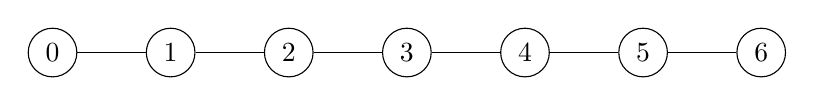
\begin{tikzpicture}
			\node[circle, draw = black] at (0,0) (n0) {0};
			\node[circle, draw = black] at (1.5,0) (n1) {1};
			\node[circle, draw = black] at (3,0) (n2) {2};
			\node[circle, draw = black] at (4.5,0) (n3) {3};
			\node[circle, draw = black] at (6,0) (n4) {4};
			\node[circle, draw = black] at (7.5,0) (n5) {5};
			\node[circle, draw = black] at (9,0) (n6) {6};
			
			\draw (n0) -- (n1) -- (n2) -- (n3) -- (n4) -- (n5) -- (n6);
		\end{tikzpicture}
	\end{center}
	Kanten entfernt:
	\begin{center}
		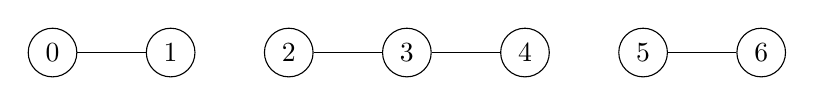
\begin{tikzpicture}
			\node[circle, draw = black] at (0,0) (n0) {0};
			\node[circle, draw = black] at (1.5,0) (n1) {1};
			\node[circle, draw = black] at (3,0) (n2) {2};
			\node[circle, draw = black] at (4.5,0) (n3) {3};
			\node[circle, draw = black] at (6,0) (n4) {4};
			\node[circle, draw = black] at (7.5,0) (n5) {5};
			\node[circle, draw = black] at (9,0) (n6) {6};
			
			\draw (n0) -- (n1);
			\draw (n2) -- (n3) -- (n4);
			\draw (n5) -- (n6);
		\end{tikzpicture}
	\end{center}
	neu verbunden:
	\begin{center}
		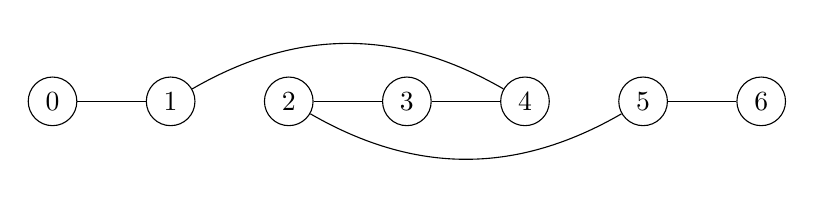
\begin{tikzpicture}
			\node[circle, draw = black] at (0,0) (n0) {0};
			\node[circle, draw = black] at (1.5,0) (n1) {1};
			\node[circle, draw = black] at (3,0) (n2) {2};
			\node[circle, draw = black] at (4.5,0) (n3) {3};
			\node[circle, draw = black] at (6,0) (n4) {4};
			\node[circle, draw = black] at (7.5,0) (n5) {5};
			\node[circle, draw = black] at (9,0) (n6) {6};
			
			\draw (n0) -- (n1);
			\draw  (n2) -- (n3) -- (n4);
			\draw (n5) -- (n6);
			\draw (n1) to[bend left=30] (n4);
			\draw (n2) to[bend right=30] (n5);
		\end{tikzpicture}
	\end{center}
	Führt zu
	\begin{align}
		M(\text{2-EdgeExchange}, s, 1, 4) = [0, 1, 4, 3, 2 , 5 , 6] \notag
	\end{align}
	
	\section*{Aufgabe 2: Theorie II: TwoEdgeExchange Move}
	\begin{enumerate}[label=(\alph*)]
		\item Wären $i$ und $j$ nur 1 voneinander entfernt, so wären sie benachtbart $\to$ kein TwoEdgeExchange-Move \\
		Wären $i$ und $j$ nur 2 voneinander entfernt, so gibt es nur ein Element in der "Mitte" und der TwoEdgeExchange-Move entspricht einem Swap-Move. \\
		$\Rightarrow$ $i$ und $j$ müssen mindestens 3 voneinander entfernt sein
		\item In einer Sequenz gibt es $n-1$ Kanten. \\
		Wenn ich die erste Kante entferne, dann habe ich noch $n-1-2 = n-3$ Kanten, die ich auch entfernen könnte. \\
		Wenn ich die zweite Kante entferne, dann habe ich noch $n-4$ Kanten, die ich auch entfernen könnte. \\
		Wenn ich die dritte Kante entferne, dann habe ich noch $n-5$ Kanten, die ich auch entfernen könnte. \\
		Wenn ich die vierte Kante entferne, dann habe ich noch $n-5$ Kanten ($n-6$ Kanten rechts davon, eine mögliche Kante links davon), die ich auch entfernen könnte. \\
		Wenn ich die fünfte Kante entferne, dann habe ich noch $n-5$ Kanten ($n-7$ Kanten rechts davon, zwei mögliche Kanten links davon), die ich auch entfernen könnte. \\
		$\dots$ \\
		Wenn ich die $(n-3)$-te Kante entferne, dann habe ich noch $n-5$ Kanten ($n-6$ links, eine rechts), die ich entfernen könnte. \\
		Wenn ich die $(n-2)$-te Kante entferne, dann habe ich noch $n-5$ Kanten, die ich links davon entfernen könnte. \\
		Wenn ich die $(n-1)$-te Kante entferne, dann habe ich noch $n-4$ Kanten, die ich links davon entfernen könnte. \\
		Wenn ich die $n$-te Kante entferne, dann habe ich noch $n-3$ Kanten, die ich links davon entfernen könnte. \\
		$\Rightarrow 2(n-3) + 2(n-4) + (n-4)(n-5)$ Möglichkeiten, aber wenn $i>j$, dann ändert sich die Permutation nicht \\
		$\Rightarrow |N(\text{2-EdgeExchange}, s)| = (n-3) + (n-4) + \frac{1}{2}(n-4)(n-5)$
	\end{enumerate}

	\section*{Aufgabe 3: Implementierung: TwoEdgeExchange-Move}
	Hinzugefügter Code in \texttt{Neighborhood.py}
	\begin{lstlisting}
class TwoEdgeExchangeMove:
	def __init__(self, initialPermutation, indexA, indexB):
		self.Permutation = list(initialPermutation)
		list1 = initialPermutation[:indexA]
		list2 = initialPermutation[indexA:indexB]
		list3 = initialPermutation[indexB:]
		self.Permutation = list1 + list(reversed(list2)) + list3

class TwoEdgeExchangeNeighborhood(BaseNeighborhood):
	def __init__(self, inputData, initialPermutation, evaluationLogic, solutionPool):
		super().__init__(inputData, initialPermutation, evaluationLogic, solutionPool)
		self.Type = "TwoEdgeExchange"

	def DiscoverMoves(self):
		for i in range(1, len(self.Permutation)):
			for j in range(1, len(self.Permutation)):
				if j-i >= 3 and j > i:
					twoEdgeExchangeMove = TwoEdgeExchangeMove(self.Permutation, i, j)
					self.Moves.append(twoEdgeExchangeMove)
	\end{lstlisting}
	Aktualisierter Code in \texttt{ImprovementAlgorithm.py}
	\begin{lstlisting}
def CreateNeighborhood(self, neighborhoodType, bestCurrentSolution):
	if neighborhoodType == 'Swap':
		return SwapNeighborhood(self.InputData, bestCurrentSolution.Permutation, self.EvaluationLogic, self.SolutionPool)
	elif neighborhoodType == 'Insertion':
		return InsertionNeighborhood(self.InputData, bestCurrentSolution.Permutation, self.EvaluationLogic, self.SolutionPool)
	elif neighborhoodType == 'TwoEdgeExchange':
		return TwoEdgeExchangeNeighborhood(self.InputData, bestCurrentSolution.Permutation, self.EvaluationLogic, self.SolutionPool)
	else:
		raise Exception(f"Neighborhood type {neighborhoodType} not defined.")

	\end{lstlisting}

\end{document}